\chapter{Future Work}

While current work has contributed towards modelling plates using spring ball system through an energy minimization. In addition to helping in prediction of deflection and other relevant quantities for complex loading, shape and other conditions, this project can be continued to study the following promising fields some of which pave the way for deployable Structures while others guide towards the development of metamaterials with interesting mechanical properties.

\section{Form Finding}
This will involve studying the shapes that lattice takes under different stimulus such tweaking the spring lengths, varying stiffness of the springs, providing pre-tensions in the spring and so on. This will be used to induce curvature, morphing into different shapes and so on.\cite{DU2020103370}\cite{Jones_2015}

\begin{figure}[!htbp]
    \centering
    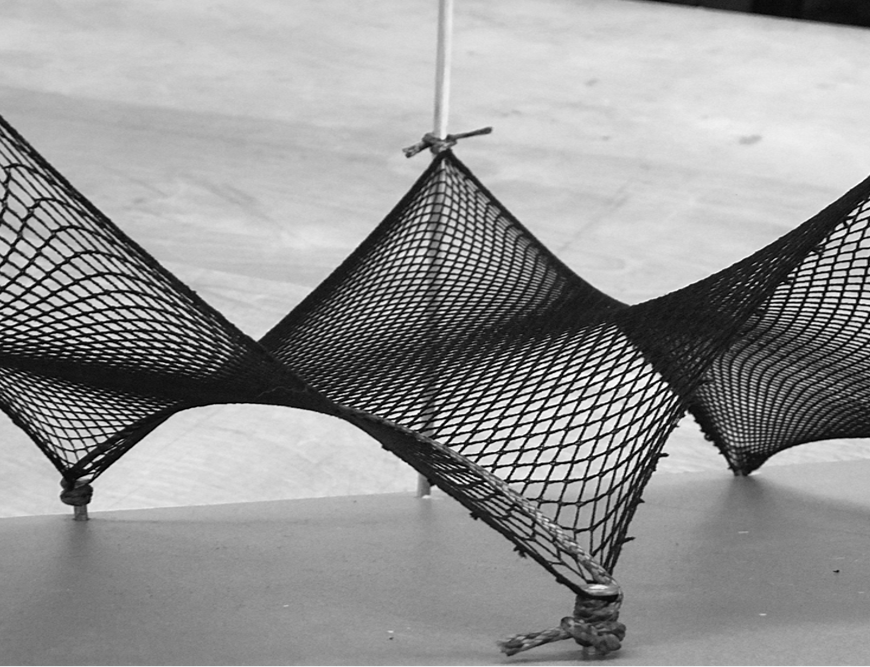
\includegraphics[width = 1\textwidth]{Figures/form_finding.png}
\end{figure}

\section{Vibration Modes \& Wave Propagation}
Using the concepts of reciprocal lattice in addition to the program, the phonon modes of the structure and other relevant lattice characteristics can be determined which will provide insights into the vibrational modes of lattice and wave propagation characteristic of the lattice. This model will aid in understanding the effect of selective pre-stress and topology on the static and dynamic property of the model.\cite{Ma}
\begin{figure}[!htbp]
    \centering
    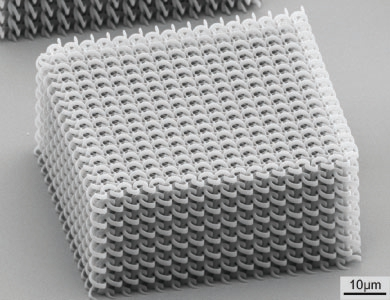
\includegraphics[width = 1\textwidth]{Figures/wave_prop_metamterials.jpg}
\end{figure}
